\documentclass[tikz,border=10pt]{standalone}
\usepackage{tikz}
\usetikzlibrary{shapes.geometric, arrows.meta, positioning}

\tikzstyle{input} = [rectangle, minimum width=3cm, minimum height=1cm, text centered, draw=black]
\tikzstyle{block} = [rectangle, minimum width=3cm, minimum height=1cm, text centered, draw=black, fill=blue!30]
\tikzstyle{output} = [rectangle, minimum width=3cm, minimum height=1cm, text centered, draw=black, fill=orange!30]
\tikzstyle{arrow} = [thick,->,>=stealth]

\begin{document}
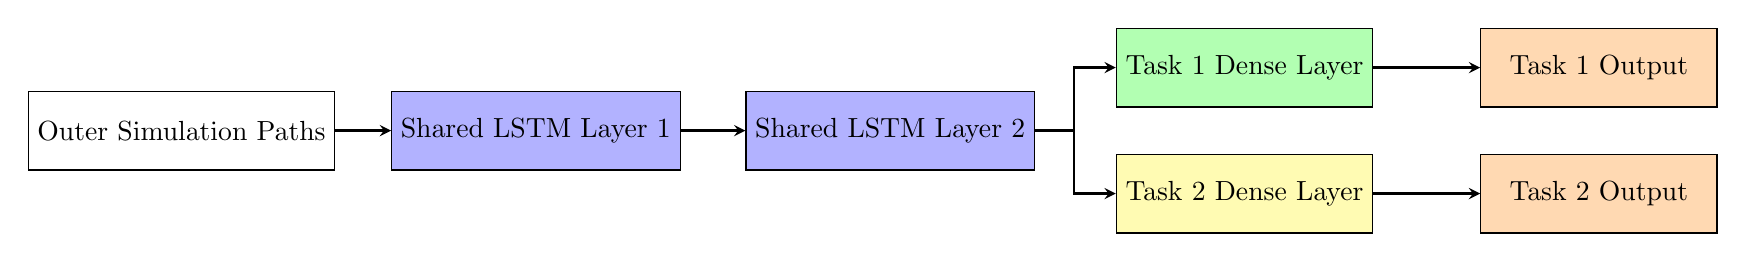
\begin{tikzpicture}[node distance=2cm]

    % Input layers
    \node (input1) [input] {Outer Simulation Paths};

    % Shared LSTM layers
    \node (lstm1) [block, right of=input1, xshift=2.5cm] {Shared LSTM Layer 1};
    \node (lstm2) [block, right of=lstm1, xshift=2.5cm] {Shared LSTM Layer 2};

    % Task-specific dense layers (Task 1)
    \node (dense1) [block, right of=lstm2, xshift=2.5cm, yshift=0.8cm, fill=green!30] {Task 1 Dense Layer};
    \node (output1) [output, right of=dense1, xshift=2.5cm] {Task 1 Output};

    % Task-specific dense layers (Task 2)
    \node (dense2) [block, right of=lstm2, xshift=2.5cm, yshift=-0.8cm, fill=yellow!30] {Task 2 Dense Layer};
    \node (output2) [output, right of=dense2, xshift=2.5cm] {Task 2 Output};

    % Arrows
    \draw [arrow] (input1) -- (lstm1);

    \draw [arrow] (lstm1) -- (lstm2);

    \draw [arrow] (lstm2.east) -- ++(0.5,0) |- (dense1.west);
    \draw [arrow] (lstm2.east) -- ++(0.5,0) |- (dense2.west);

    \draw [arrow] (dense1) -- (output1);
    \draw [arrow] (dense2) -- (output2);

\end{tikzpicture}
\end{document}
